\documentclass[]{article}
\usepackage{lmodern}
\usepackage{amssymb,amsmath}
\usepackage{ifxetex,ifluatex}
\usepackage{fixltx2e} % provides \textsubscript
\ifnum 0\ifxetex 1\fi\ifluatex 1\fi=0 % if pdftex
  \usepackage[T1]{fontenc}
  \usepackage[utf8]{inputenc}
\else % if luatex or xelatex
  \ifxetex
    \usepackage{mathspec}
    \usepackage{xltxtra,xunicode}
  \else
    \usepackage{fontspec}
  \fi
  \defaultfontfeatures{Mapping=tex-text,Scale=MatchLowercase}
  \newcommand{\euro}{€}
\fi
% use upquote if available, for straight quotes in verbatim environments
\IfFileExists{upquote.sty}{\usepackage{upquote}}{}
% use microtype if available
\IfFileExists{microtype.sty}{%
\usepackage{microtype}
\UseMicrotypeSet[protrusion]{basicmath} % disable protrusion for tt fonts
}{}
\usepackage[margin=1in]{geometry}
\usepackage{color}
\usepackage{fancyvrb}
\newcommand{\VerbBar}{|}
\newcommand{\VERB}{\Verb[commandchars=\\\{\}]}
\DefineVerbatimEnvironment{Highlighting}{Verbatim}{commandchars=\\\{\}}
% Add ',fontsize=\small' for more characters per line
\usepackage{framed}
\definecolor{shadecolor}{RGB}{248,248,248}
\newenvironment{Shaded}{\begin{snugshade}}{\end{snugshade}}
\newcommand{\KeywordTok}[1]{\textcolor[rgb]{0.13,0.29,0.53}{\textbf{{#1}}}}
\newcommand{\DataTypeTok}[1]{\textcolor[rgb]{0.13,0.29,0.53}{{#1}}}
\newcommand{\DecValTok}[1]{\textcolor[rgb]{0.00,0.00,0.81}{{#1}}}
\newcommand{\BaseNTok}[1]{\textcolor[rgb]{0.00,0.00,0.81}{{#1}}}
\newcommand{\FloatTok}[1]{\textcolor[rgb]{0.00,0.00,0.81}{{#1}}}
\newcommand{\CharTok}[1]{\textcolor[rgb]{0.31,0.60,0.02}{{#1}}}
\newcommand{\StringTok}[1]{\textcolor[rgb]{0.31,0.60,0.02}{{#1}}}
\newcommand{\CommentTok}[1]{\textcolor[rgb]{0.56,0.35,0.01}{\textit{{#1}}}}
\newcommand{\OtherTok}[1]{\textcolor[rgb]{0.56,0.35,0.01}{{#1}}}
\newcommand{\AlertTok}[1]{\textcolor[rgb]{0.94,0.16,0.16}{{#1}}}
\newcommand{\FunctionTok}[1]{\textcolor[rgb]{0.00,0.00,0.00}{{#1}}}
\newcommand{\RegionMarkerTok}[1]{{#1}}
\newcommand{\ErrorTok}[1]{\textbf{{#1}}}
\newcommand{\NormalTok}[1]{{#1}}
\usepackage{graphicx}
\makeatletter
\def\maxwidth{\ifdim\Gin@nat@width>\linewidth\linewidth\else\Gin@nat@width\fi}
\def\maxheight{\ifdim\Gin@nat@height>\textheight\textheight\else\Gin@nat@height\fi}
\makeatother
% Scale images if necessary, so that they will not overflow the page
% margins by default, and it is still possible to overwrite the defaults
% using explicit options in \includegraphics[width, height, ...]{}
\setkeys{Gin}{width=\maxwidth,height=\maxheight,keepaspectratio}
\ifxetex
  \usepackage[setpagesize=false, % page size defined by xetex
              unicode=false, % unicode breaks when used with xetex
              xetex]{hyperref}
\else
  \usepackage[unicode=true]{hyperref}
\fi
\hypersetup{breaklinks=true,
            bookmarks=true,
            pdfauthor={Ben Arancibia},
            pdftitle={IS 622 Week 8 Homework},
            colorlinks=true,
            citecolor=blue,
            urlcolor=blue,
            linkcolor=magenta,
            pdfborder={0 0 0}}
\urlstyle{same}  % don't use monospace font for urls
\setlength{\parindent}{0pt}
\setlength{\parskip}{6pt plus 2pt minus 1pt}
\setlength{\emergencystretch}{3em}  % prevent overfull lines
\setcounter{secnumdepth}{0}

%%% Use protect on footnotes to avoid problems with footnotes in titles
\let\rmarkdownfootnote\footnote%
\def\footnote{\protect\rmarkdownfootnote}

%%% Change title format to be more compact
\usepackage{titling}

% Create subtitle command for use in maketitle
\newcommand{\subtitle}[1]{
  \posttitle{
    \begin{center}\large#1\end{center}
    }
}

\setlength{\droptitle}{-2em}
  \title{IS 622 Week 8 Homework}
  \pretitle{\vspace{\droptitle}\centering\huge}
  \posttitle{\par}
  \author{Ben Arancibia}
  \preauthor{\centering\large\emph}
  \postauthor{\par}
  \predate{\centering\large\emph}
  \postdate{\par}
  \date{October 18, 2015}



\begin{document}

\maketitle


\textbf{7.1.3}

Suppose we have a d-dimensional Euclidean space. Consider vectors whose
components are only +1 or −1 in each dimension. Note that each vector
has length d\^{}(1/2), so the product of their lengths (denominator in
the formula for the cosine of the angle between them) is d. If we chose
each component independently, and a component is as likely to be +1 as
−1, what is the distribution of the value of the numerator of the
formula (i.e., the sum of the products of the corresponding components
from each vector)? What can you say about the expected value of the
cosine of the angle between the vectors, as d grows large?

If we have a d-dimensional Euclidean space, a problem exists of ``curse
of dimensionality''. In high dimensions almost all pairs are equally far
away from one other. As defined in the problem, you have two equally
likely possibilitys +1 and -1. Since they are equally likely the value
of the summing would be 0 (1 + -1 = 0). For large d, the cosine of an
angle is close to 0 because the summation is 0. If the cosine of an
angle is 0 then the angle has to be close to 90 degrees.

\textbf{7.2.1}

Perform a hierarchical clustering of the one-dimensional set of points
1, 4, 9, 16, 25, 36, 49, 64, 81, assuming clusters are represented by
their centroid (average), and at each step the clusters with the closest
centroids are merged.

\begin{Shaded}
\begin{Highlighting}[]
\NormalTok{clusters <-}\StringTok{ }\KeywordTok{list}\NormalTok{( }\KeywordTok{c}\NormalTok{(}\DecValTok{1}\NormalTok{), }\KeywordTok{c}\NormalTok{(}\DecValTok{4}\NormalTok{), }\KeywordTok{c}\NormalTok{(}\DecValTok{9}\NormalTok{), }\KeywordTok{c}\NormalTok{(}\DecValTok{16}\NormalTok{), }\KeywordTok{c}\NormalTok{(}\DecValTok{25}\NormalTok{), }\KeywordTok{c}\NormalTok{(}\DecValTok{36}\NormalTok{), }\KeywordTok{c}\NormalTok{(}\DecValTok{49}\NormalTok{), }\KeywordTok{c}\NormalTok{(}\DecValTok{64}\NormalTok{), }\KeywordTok{c}\NormalTok{(}\DecValTok{81}\NormalTok{))}

\NormalTok{hc <-}\StringTok{ }\KeywordTok{hclust}\NormalTok{(}\KeywordTok{dist}\NormalTok{(clusters), }\StringTok{"cen"}\NormalTok{)}
\NormalTok{hc$merge}
\end{Highlighting}
\end{Shaded}

\begin{verbatim}
##      [,1] [,2]
## [1,]   -1   -2
## [2,]   -3    1
## [3,]   -4   -5
## [4,]    2    3
## [5,]   -6   -7
## [6,]   -8   -9
## [7,]    5    6
## [8,]    4    7
\end{verbatim}

\begin{Shaded}
\begin{Highlighting}[]
\KeywordTok{plot}\NormalTok{(hc, }\DataTypeTok{main =} \StringTok{"From 9 clusters to 1, Follow tree up"}\NormalTok{)}
\end{Highlighting}
\end{Shaded}

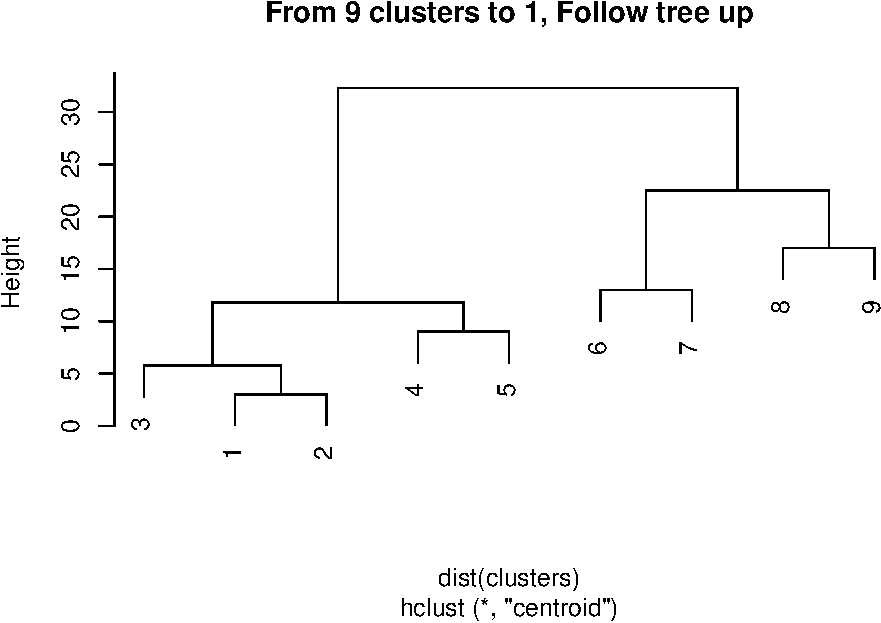
\includegraphics{arancibia_week8_hw_files/figure-latex/unnamed-chunk-1-1.pdf}

\textbf{7.2.2}

How would the clustering of Example 7.2 change if we used for the
distance between two clusters:

\begin{Shaded}
\begin{Highlighting}[]
\NormalTok{points <-}\StringTok{ }\KeywordTok{c}\NormalTok{(}\DecValTok{2}\NormalTok{,}\DecValTok{2}\NormalTok{,}\DecValTok{3}\NormalTok{,}\DecValTok{4}\NormalTok{,}\DecValTok{5}\NormalTok{,}\DecValTok{2}\NormalTok{,}\DecValTok{9}\NormalTok{,}\DecValTok{3}\NormalTok{,}\DecValTok{12}\NormalTok{,}\DecValTok{3}\NormalTok{,}\DecValTok{11}\NormalTok{,}\DecValTok{4}\NormalTok{,}\DecValTok{10}\NormalTok{,}\DecValTok{5}\NormalTok{,}\DecValTok{12}\NormalTok{,}\DecValTok{6}\NormalTok{,}\DecValTok{6}\NormalTok{,}\DecValTok{8}\NormalTok{,}\DecValTok{4}\NormalTok{,}\DecValTok{8}\NormalTok{,}\DecValTok{4}\NormalTok{,}\DecValTok{10}\NormalTok{,}\DecValTok{7}\NormalTok{,}\DecValTok{10}\NormalTok{)}
\NormalTok{points <-}\StringTok{ }\KeywordTok{matrix}\NormalTok{(points, }\DataTypeTok{nrow=}\DecValTok{12}\NormalTok{, }\DataTypeTok{ncol=}\DecValTok{2}\NormalTok{, }\DataTypeTok{byrow=}\OtherTok{TRUE}\NormalTok{)}
\NormalTok{points <-}\StringTok{ }\KeywordTok{as.data.frame}\NormalTok{(points)}

\NormalTok{points}
\end{Highlighting}
\end{Shaded}

\begin{verbatim}
##    V1 V2
## 1   2  2
## 2   3  4
## 3   5  2
## 4   9  3
## 5  12  3
## 6  11  4
## 7  10  5
## 8  12  6
## 9   6  8
## 10  4  8
## 11  4 10
## 12  7 10
\end{verbatim}

\begin{enumerate}
\def\labelenumi{(\alph{enumi})}
\itemsep1pt\parskip0pt\parsep0pt
\item
  The minimum of the distances between any two points, one from each
  cluster.
\end{enumerate}

\begin{Shaded}
\begin{Highlighting}[]
\NormalTok{hc <-}\StringTok{ }\KeywordTok{hclust}\NormalTok{(}\KeywordTok{dist}\NormalTok{(points), }\StringTok{"single"}\NormalTok{)}
\KeywordTok{plot}\NormalTok{(hc)}
\end{Highlighting}
\end{Shaded}

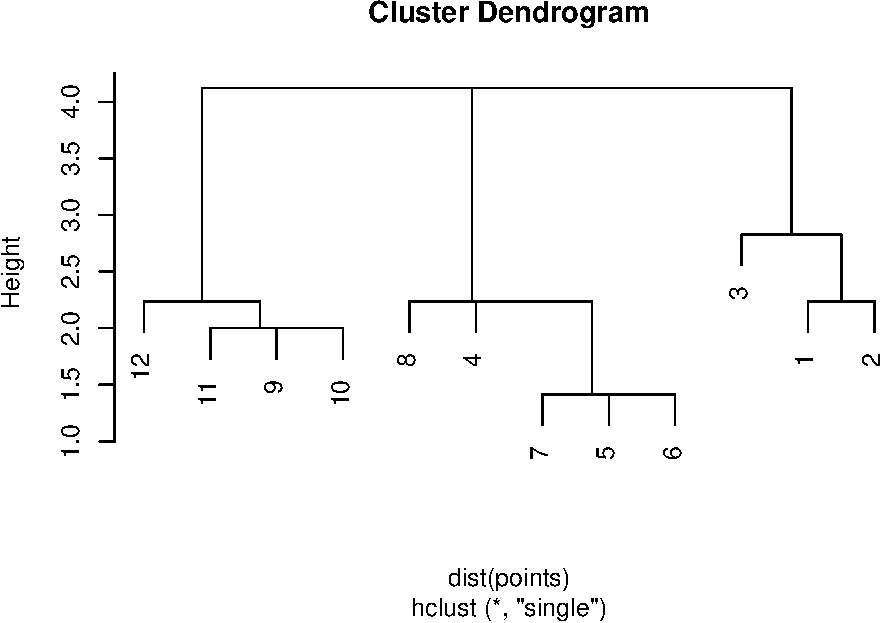
\includegraphics{arancibia_week8_hw_files/figure-latex/unnamed-chunk-3-1.pdf}

\begin{enumerate}
\def\labelenumi{(\alph{enumi})}
\setcounter{enumi}{1}
\itemsep1pt\parskip0pt\parsep0pt
\item
  The average of the distances between pairs of points, one from each of
  the two clusters.
\end{enumerate}

\begin{Shaded}
\begin{Highlighting}[]
\NormalTok{hc <-}\StringTok{ }\KeywordTok{hclust}\NormalTok{(}\KeywordTok{dist}\NormalTok{(points), }\StringTok{"average"}\NormalTok{)}
\KeywordTok{plot}\NormalTok{(hc)}
\end{Highlighting}
\end{Shaded}

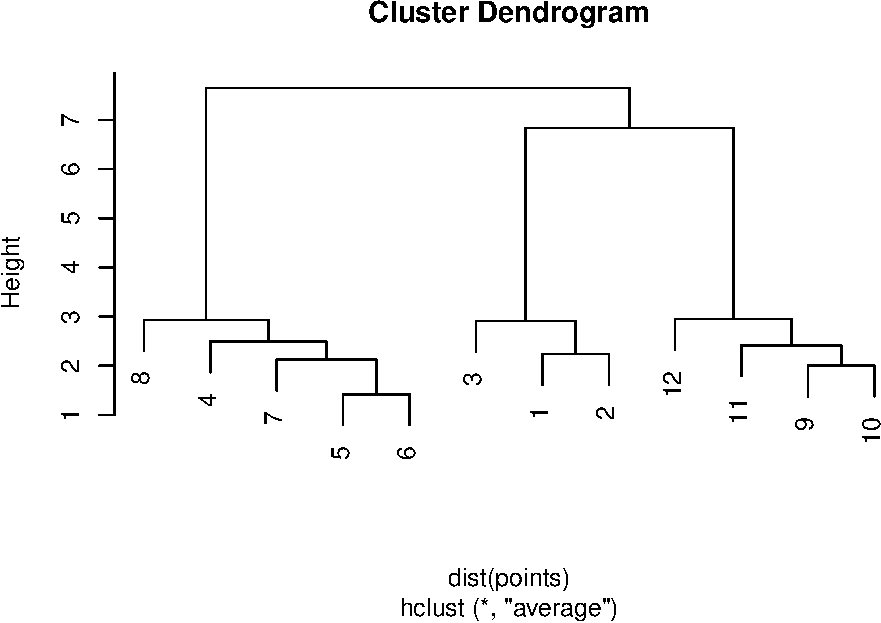
\includegraphics{arancibia_week8_hw_files/figure-latex/unnamed-chunk-4-1.pdf}

\end{document}
